\documentclass[12pt,a4paper]{report}

\usepackage[T1]{fontenc}
\usepackage[utf8]{inputenc}
\usepackage[english]{babel}
\usepackage{lmodern}
\usepackage{geometry}
\geometry{margin=2.5cm}
\usepackage{setspace}
\onehalfspacing
\usepackage{graphicx}
\usepackage{float}
\usepackage{booktabs}
\usepackage{longtable}
\usepackage{array}
\usepackage{amsmath}
\usepackage{amssymb}
\usepackage{siunitx}
\usepackage{xcolor}
\usepackage{hyperref}
\usepackage{listings}
\usepackage{tikz}
\usepackage{pgfplots}
\usepackage{caption}
\usepackage{subcaption}
\usepackage{enumitem}
\usepackage{fancyhdr}
\usepackage[numbers]{natbib}
\pgfplotsset{compat=1.18}
\usetikzlibrary{positioning,arrows.meta,shapes.geometric,fit,backgrounds}

\hypersetup{
  colorlinks=true,
  linkcolor=blue!60!black,
  urlcolor=blue!60!black,
  citecolor=blue!60!black,
  pdftitle={EcoEye2 Project Defense Report},
  pdfauthor={Project Team},
  pdfsubject={Financial ETL and Economic Adjustment Platform}
}

\lstdefinestyle{py}{
  language=Python,
  basicstyle=\ttfamily\small,
  keywordstyle=\color{blue!70!black}\bfseries,
  commentstyle=\color{green!40!black},
  stringstyle=\color{orange!60!black},
  numbers=left,
  numberstyle=\tiny\color{gray},
  stepnumber=1,
  numbersep=8pt,
  breaklines=true,
  frame=single,
  rulecolor=\color{black!20}
}

\pagestyle{fancy}
\fancyhf{}
\fancyhead[L]{EcoEye2 Project Defense}
\fancyhead[R]{\leftmark}
\fancyfoot[C]{\thepage}

\title{
  \Huge\textbf{Design and Implementation of EcoEye2}\\
  \Large A Financial ETL and Economic Adjustment Platform\\[1em]
  \large Graduation Project Report
}
\author{
  Student: \textbf{........................................} \\
  Supervisor: \textbf{........................................} \\
  Department: \textbf{........................................}
}
\date{Academic Year 2025--2026}

\begin{document}

\begin{titlepage}
  \centering
  {\Large University Name}\\[0.4cm]
  {\large Faculty / School Name}\\[1.4cm]
  {\Large\textbf{Graduation Project Defense Report}}\\[1.2cm]
  {\Huge\textbf{EcoEye2}}\\[0.2cm]
  {\Large Financial ETL Pipeline with Economic Adjustment Layer}\\[1.2cm]
  \begin{tabular}{p{0.3\textwidth}p{0.6\textwidth}}
    Student: & .................................................... \\
    Supervisor: & .................................................... \\
    Jury President: & .................................................... \\
    Jury Member: & .................................................... \\
  \end{tabular}\\[1.5cm]
  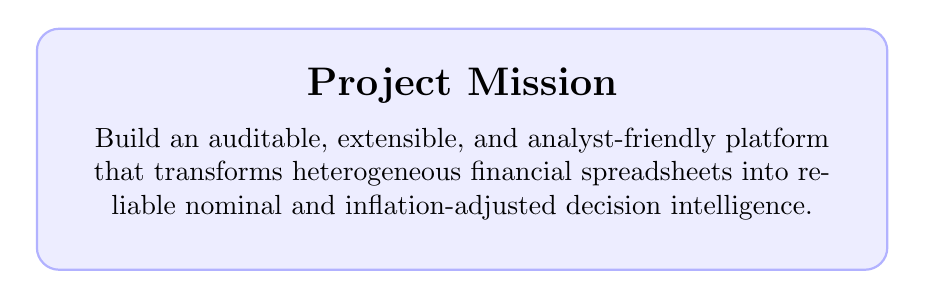
\begin{tikzpicture}[scale=0.9]
    \draw[rounded corners=8pt,fill=blue!7,draw=blue!30,line width=0.8pt] (0,0) rectangle (12,3.4);
    \node[align=center] at (6,2.6) {\Large\textbf{Project Mission}};
    \node[align=center,text width=10.8cm] at (6,1.35) {Build an auditable, extensible, and analyst-friendly platform that transforms heterogeneous financial spreadsheets into reliable nominal and inflation-adjusted decision intelligence.};
  \end{tikzpicture}\\[1.5cm]
  {\large Academic Year 2025--2026}
\end{titlepage}

\pagenumbering{roman}
\chapter*{Dedication}
This work is dedicated to our families, teachers, and all professionals who believe that data quality is the first step toward better strategic decisions.

\chapter*{Acknowledgements}
We express sincere gratitude to our project supervisor for continuous guidance, to the jury for their time and valuable remarks, and to all colleagues who contributed feedback during development and testing. We also acknowledge the maintainers of open-source technologies used in this project, including Python, FastAPI, React, and SQLite.

\chapter*{Abstract}
This report presents \textbf{EcoEye2}, a full-stack platform that automates financial data ingestion and normalization from spreadsheet sources, then enriches this data through a macroeconomic adjustment layer. The system combines an ETL pipeline, provider-aware economic indicator fetchers, and a web interface for data operations, visualization, and analysis. The key contribution is a practical architecture that preserves raw financial records while generating parallel \texttt{*\_real} tables for inflation-deflated and present-value interpretations.

The implementation supports configurable transformations, robust logging, API-driven workflows, and front-end analytics views. A hybrid methodology was followed: incremental delivery of backend modules, integration of a responsive user interface, and test-driven validation of transformation outputs. Performance observations and quality criteria indicate that the solution is suitable for small and medium organizations that require auditable financial intelligence without heavyweight infrastructure.

\chapter*{Keywords}
ETL, Financial Analytics, Inflation Adjustment, FastAPI, React, SQLite, Data Quality, Economic Indicators

\tableofcontents
\listoffigures
\listoftables

\clearpage
\pagenumbering{arabic}

\chapter{General Introduction}
\section{Context}
Organizations often keep accounting and managerial records in spreadsheets created by different teams over long periods. While spreadsheets are flexible, they also create inconsistency in naming conventions, date formats, and calculation logic. As data volume grows, manual consolidation becomes costly and error-prone. The project addressed this context by building a repeatable ETL process and a web application that transforms disconnected files into a coherent analytical model.

\section{Problem Statement}
The initial challenge was not only technical ingestion. It also involved preserving traceability and enabling meaningful interpretation of nominal financial values across changing economic conditions. A revenue value from one year cannot be compared directly with a value from another year without accounting for inflation and, in some cases, discount rates. Therefore, an end-to-end system was required with:
\begin{itemize}[leftmargin=1.5em]
  \item configurable data extraction and transformation from heterogeneous files,
  \item persistent storage with low operational overhead,
  \item transparent rules for inflation and time-value adjustment,
  \item an interface usable by non-developer stakeholders.
\end{itemize}

\section{Objectives}
The project objectives were structured in four layers:
\begin{enumerate}[leftmargin=1.5em]
  \item Build a robust ETL core capable of ingesting multiple table schemas.
  \item Implement an economic layer combining CPI/PPI deflation and present value.
  \item Expose operations through a secure API and a usable web interface.
  \item Provide visualization and reporting support for decision makers.
\end{enumerate}

\section{Report Structure}
This manuscript is organized from conceptual framing to implementation details and evaluation. After the introduction and related work perspective, it explains architecture, implementation choices, validation methodology, deployment strategy, and recommendations for future improvements.

\chapter{Background and Related Concepts}
\section{ETL in Financial Data Pipelines}
Extract, Transform, Load (ETL) remains a central paradigm for analytical systems where input quality varies across sources \citep{kimball}. In financial contexts, ETL complexity increases because records encode business semantics such as account hierarchies, period boundaries, and multi-source mappings. The project follows a modular ETL decomposition where extraction is source-specific, transformation is rule-driven, and loading is deterministic.

\section{Economic Adjustment Fundamentals}
Financial interpretation over time requires normalization. Let $A_t$ be nominal amount at period $t$, and let $D_t$ be the deflator index (CPI or PPI) normalized to base period $b$. Real value is:
\begin{equation}
  A^{real}_t = A_t \times \frac{D_b}{D_t}
\end{equation}
For discounting to reference date $T$ at annual rate $r$:
\begin{equation}
  A^{pv}_t = \frac{A_t}{(1+r)^{\Delta t}}
\end{equation}
where $\Delta t$ is expressed in years. Combining these views allows managers to compare values consistently.

\section{Technology Positioning}
The chosen stack emphasizes maintainability and accessibility:
\begin{itemize}[leftmargin=1.5em]
  \item \textbf{Python} for data operations and API logic.
  \item \textbf{SQLite} for embedded persistence with simple deployment.
  \item \textbf{FastAPI} for typed, documented REST interfaces.
  \item \textbf{React + Vite} for responsive front-end workflows.
\end{itemize}
This combination balances development speed and production pragmatism for small to medium scope deployments.

\chapter{Requirements and Analysis}
\section{Functional Requirements}
Key expected capabilities were:
\begin{enumerate}[leftmargin=1.5em]
  \item Upload and register raw input workbooks.
  \item Execute ETL for all tables or selected subsets.
  \item Persist transformed data to database and optional Parquet outputs.
  \item Fetch macro indicators from prioritized data providers.
  \item Generate parallel real-value tables without overwriting nominal data.
  \item Expose data editing and analytics views through web UI.
\end{enumerate}

\section{Non-Functional Requirements}
The system had to remain:
\begin{itemize}[leftmargin=1.5em]
  \item \textbf{Auditable}: each transformation path should be reproducible.
  \item \textbf{Extensible}: new sources and transform types can be added with minimal friction.
  \item \textbf{Reliable}: clear error propagation and log outputs.
  \item \textbf{Usable}: workflows should be executable by analysts with limited coding background.
\end{itemize}

\section{Constraints}
The project timeline and infrastructure constraints encouraged an architecture with low setup complexity. Existing spreadsheet variability required a configuration-first approach rather than hardcoded source assumptions.

\chapter{System Architecture}
\section{High-Level Architecture}
\begin{figure}[H]
\centering
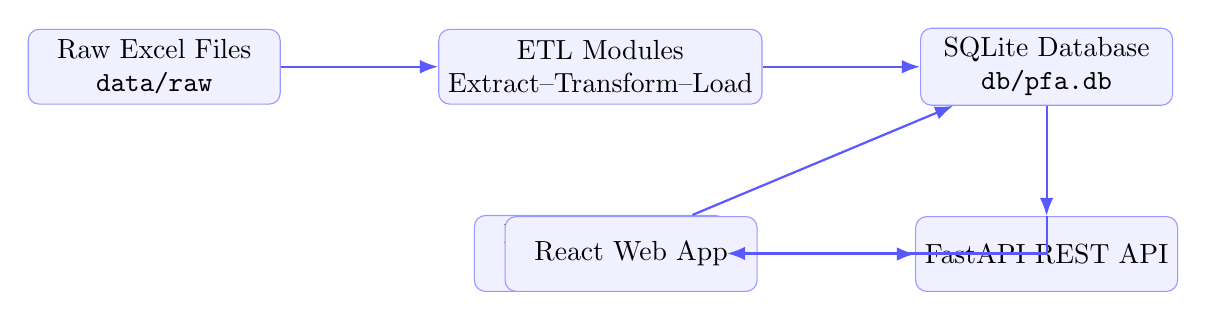
\begin{tikzpicture}[
  node distance=1.4cm,
  box/.style={rectangle, rounded corners, draw=blue!40, fill=blue!6, minimum width=3.2cm, minimum height=0.95cm, align=center},
  arr/.style={-Latex, thick, blue!65}
]
\node[box] (raw) {Raw Excel Files\\\texttt{data/raw}};
\node[box, right=2.0cm of raw] (etl) {ETL Modules\\Extract--Transform--Load};
\node[box, right=2.0cm of etl] (db) {SQLite Database\\\texttt{db/pfa.db}};
\node[box, below=1.4cm of etl] (econ) {Economic Layer\\Fetch + Apply};
\node[box, below=1.4cm of db] (api) {FastAPI REST API};
\node[box, left=2.0cm of api] (web) {React Web App};

\draw[arr] (raw) -- (etl);
\draw[arr] (etl) -- (db);
\draw[arr] (econ) -- (db);
\draw[arr] (db) -- (api);
\draw[arr] (web) -- (api);
\draw[arr] (api) |- (econ);
\end{tikzpicture}
\caption{EcoEye2 macro architecture.}
\end{figure}

\section{Data Lifecycle}
Data enters through source files and exits as validated analytical tables. The lifecycle deliberately keeps raw and real-value representations separated. This protects traceability and allows users to audit adjustment effects.

\section{Configuration-Driven Extensibility}
Source metadata and transformation behavior are expressed in configuration modules. This eliminates repeated code changes for every new workbook and allows incremental onboarding of business units.

\section{Security Envelope}
For mutable API routes, an optional API key header can be activated. While simple, this mechanism provides a practical first barrier in internal deployments and can be extended later with identity providers.

\chapter{Implementation}
\section{ETL Core Implementation}
The ETL entry script orchestrates table-level processing either globally or for a single target. Extraction reads declared sheets and ranges; transformation normalizes schema and values; loading writes stable outputs.

\begin{lstlisting}[style=py, caption={Simplified ETL launcher behavior.}]
if len(sys.argv) > 1:
    result = run_etl_single(sys.argv[1])
else:
    result = run_etl_all()
\end{lstlisting}

Supported transform types include transactional, budget, balance sheet, mapping, aging, time series, and generic. This taxonomy covers most finance-office datasets observed during project scoping.

\section{Economic Indicator Fetch and Application}
The economic layer fetches indicators through a provider chain (HCP, FRED, World Bank, BAM depending on availability). Indicator history is stored in \texttt{econ\_indicators}. The apply phase then produces \texttt{*\_real} tables and adds analytical fields such as:
\begin{itemize}[leftmargin=1.5em]
  \item \texttt{cpi\_deflator} or \texttt{ppi\_deflator},
  \item \texttt{amount\_real\_<base\_period>},
  \item \texttt{amount\_pv\_<reference\_date>}.
\end{itemize}

\begin{lstlisting}[style=py, caption={Economic workflow command pattern.}]
python run_econ.py fetch
python run_econ.py apply
python run_econ.py all
\end{lstlisting}

\section{Backend API}
FastAPI was selected for explicit request/response validation and automatic OpenAPI documentation. API routes expose pipeline control, analytics access, table browsing, and uploads. This explicit contract reduced front-end integration ambiguity and improved testing.

\section{Frontend Application}
The React interface organizes workflows into domain pages such as ingest, data browsing, adjustments, insights, and visualization. A key design decision was to keep operations discoverable and task-oriented rather than menu-heavy.

\section{Observability and Logging}
Both ETL and economic scripts initialize logging with file and console handlers. Logs include run status and errors, enabling diagnosis without deep debugging sessions. This is especially useful in data projects where input quality is unpredictable.

\chapter{Data Model and Processing Semantics}
\section{Nominal vs Real Data Strategy}
The project follows a \emph{parallel-table strategy}. Instead of mutating original tables, adjusted results are materialized in separate tables with a \texttt{\_real} suffix. Advantages include:
\begin{itemize}[leftmargin=1.5em]
  \item immutable nominal history,
  \item simple side-by-side comparison,
  \item easier rollback and validation.
\end{itemize}

\section{Indicator Chain Fallback Logic}
Provider fallback mitigates dependency risk. If one source is unavailable or incomplete, the system attempts subsequent providers based on configured priority. This resilience is essential for routine reporting workflows.

\section{Transformation Robustness}
Transformers include schema cleanup, deduplication, date normalization, and shape conversion (wide-to-long for periodic columns). These operations improve analytical consistency across independently managed files.

\begin{figure}[H]
\centering
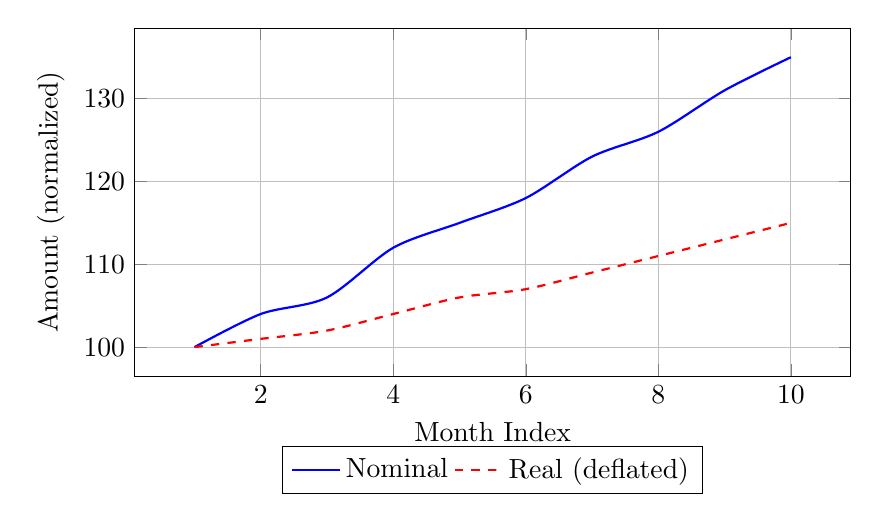
\begin{tikzpicture}
\begin{axis}[
  width=0.88\textwidth,
  height=6cm,
  xlabel=Month Index,
  ylabel=Amount (normalized),
  legend style={at={(0.5,-0.2)},anchor=north,legend columns=2},
  grid=major
]
\addplot[smooth,blue,thick] coordinates {
  (1,100) (2,104) (3,106) (4,112) (5,115) (6,118) (7,123) (8,126) (9,131) (10,135)
};
\addlegendentry{Nominal}
\addplot[smooth,red,thick,dashed] coordinates {
  (1,100) (2,101) (3,102) (4,104) (5,106) (6,107) (7,109) (8,111) (9,113) (10,115)
};
\addlegendentry{Real (deflated)}
\end{axis}
\end{tikzpicture}
\caption{Illustrative nominal vs real trend behavior.}
\end{figure}

\chapter{Validation and Results}
\section{Validation Approach}
Validation combined script-level checks, database spot verification, and UI-driven exploratory tests. The focus was not only correctness of values but also interpretability and reproducibility.

\section{Test Scenarios}
\begin{longtable}{p{0.28\textwidth}p{0.2\textwidth}p{0.45\textwidth}}
\toprule
\textbf{Scenario} & \textbf{Layer} & \textbf{Expected Result} \\
\midrule
Single-table ETL run & ETL & Selected table processed with success log and row count. \\
Full ETL run & ETL & All configured tables persisted without schema conflicts. \\
Indicator fetch with fallback & Econ & Missing provider gracefully replaced by next source in chain. \\
Apply real-value tables & Econ & \texttt{*\_real} tables created with deflator and PV columns. \\
Mutating API with key enabled & API & Request rejected when \texttt{X-Api-Key} is absent or invalid. \\
Nominal/real chart rendering & UI & User can compare trajectories visually without manual SQL. \\
\bottomrule
\caption{Representative functional validation scenarios.}
\end{longtable}

\section{Qualitative Outcomes}
The platform demonstrates clear productivity gains in repetitive financial consolidation tasks. Analysts move from fragmented spreadsheets to centralized, queryable data with less manual correction. The introduction of real-value tables improves the quality of temporal comparisons during strategic meetings.

\section{Performance Discussion}
SQLite and local file processing proved adequate for the project scale. Most runtime variability came from source file quality and external macro-provider response times. For larger deployments, caching, job queues, and asynchronous fetching can further improve throughput.

\chapter{Deployment, Operations, and Risk Management}
\section{Development and Production Modes}
The system supports:
\begin{itemize}[leftmargin=1.5em]
  \item a development mode with separate API and Vite servers,
  \item a production mode where built static assets are served by FastAPI.
\end{itemize}
Container support via Docker Compose streamlines local reproducibility.

\section{Operational Risks}
\begin{enumerate}[leftmargin=1.5em]
  \item \textbf{Input drift}: source files change structure unexpectedly.
  \item \textbf{Provider instability}: macro sources may be temporarily unavailable.
  \item \textbf{Human edits}: direct database edits can break assumptions.
\end{enumerate}
Mitigation relies on explicit config versioning, fallback chains, and log-based diagnostics.

\section{Scalability Considerations}
Future scaling options include replacing SQLite with PostgreSQL, introducing worker queues for heavy ETL jobs, and adding role-based access control for multi-user governance.

\chapter{Project Management and Methodology}
\section{Execution Strategy}
An incremental approach was adopted:
\begin{enumerate}[leftmargin=1.5em]
  \item Build ETL MVP and validate with sample data.
  \item Add economic fetch/apply capabilities.
  \item Integrate API endpoints and front-end workflows.
  \item Iterate through user feedback and reliability hardening.
\end{enumerate}

\section{Timeline Overview}
\begin{figure}[H]
\centering
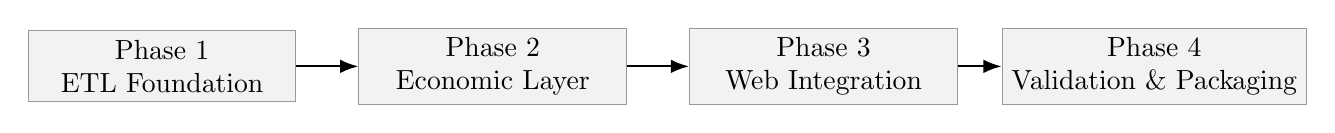
\begin{tikzpicture}[
  milestone/.style={rectangle, draw=black!40, fill=gray!10, minimum width=3.4cm, minimum height=0.9cm, align=center},
  link/.style={-Latex, thick}
]
\node[milestone] (m1) at (0,0) {Phase 1\\ETL Foundation};
\node[milestone] (m2) at (4.2,0) {Phase 2\\Economic Layer};
\node[milestone] (m3) at (8.4,0) {Phase 3\\Web Integration};
\node[milestone] (m4) at (12.6,0) {Phase 4\\Validation \& Packaging};
\draw[link] (m1) -- (m2);
\draw[link] (m2) -- (m3);
\draw[link] (m3) -- (m4);
\end{tikzpicture}
\caption{Project delivery timeline by major phases.}
\end{figure}

\section{Lessons Learned}
Three lessons were decisive:
\begin{itemize}[leftmargin=1.5em]
  \item Data projects need early investment in schema conventions.
  \item Traceability is as important as algorithmic sophistication.
  \item User experience directly affects analytical adoption.
\end{itemize}

\chapter{General Conclusion and Perspectives}
\section{Conclusion}
EcoEye2 achieved its central objective: transforming heterogeneous spreadsheet-based financial data into a coherent, auditable analytical platform enhanced by economic normalization. The system bridges operational reporting and macro-aware interpretation through an architecture that is both practical and extensible.

\section{Contributions}
Major contributions include:
\begin{enumerate}[leftmargin=1.5em]
  \item a configurable ETL pipeline for multiple financial table archetypes,
  \item a provider-chained macroeconomic fetch and adjustment workflow,
  \item a full-stack interface for ingestion, control, and visualization,
  \item a deployment model accessible to limited-resource environments.
\end{enumerate}

\section{Future Work}
Recommended extensions:
\begin{itemize}[leftmargin=1.5em]
  \item predictive analytics and anomaly detection modules,
  \item stronger authentication and role management,
  \item automated data-quality scoring at ingestion,
  \item CI-backed regression testing for transformation rules.
\end{itemize}

\appendix
\chapter{User Guide for Jury Demonstration}
\section{Demo Preparation}
To prepare a live defense demo:
\begin{enumerate}[leftmargin=1.5em]
  \item Install dependencies with \texttt{pip install -r requirements.txt}.
  \item Start API server using \texttt{python run\_ecoeye2.py}.
  \item Start web app in \texttt{ecoeye2/web} with \texttt{npm run dev}.
  \item Open the interface and execute one ETL operation.
  \item Run economic adjustment and show nominal vs real comparison.
\end{enumerate}

\section{Recommended Jury Walkthrough}
The most convincing sequence is: ingest source, run ETL, inspect a transformed table, execute economic adjustment, and conclude with chart comparison. This order highlights both engineering rigor and business value.

\chapter{API and Configuration Excerpts}
\section{Example Source Configuration}
\begin{lstlisting}[style=py]
SOURCES = {
    "my_report.xlsx": {
        "revenue": {
            "sheet_name": "Sheet1",
            "header_row": 0,
            "usecols": "A:F",
            "transform_type": "transactional",
        }
    }
}
\end{lstlisting}

\section{Example Environment Variables}
\begin{longtable}{p{0.3\textwidth}p{0.62\textwidth}}
\toprule
\textbf{Variable} & \textbf{Purpose} \\
\midrule
\texttt{ECOEYE2\_DB\_PATH} & Location of SQLite database file. \\
\texttt{ECOEYE2\_RAW\_DIR} & Directory for uploaded raw workbooks. \\
\texttt{ECOEYE2\_API\_KEY} & Key required by mutating API endpoints when enabled. \\
\texttt{FRED\_API\_KEY} & Credential for FRED CPI series fallback. \\
\bottomrule
\caption{Operational environment variables.}
\end{longtable}

\chapter{Extended Discussion for Defense Questions}
\section{Why Keep SQLite Instead of Immediate Migration to PostgreSQL?}
The database decision was driven by the project scope and operational context. SQLite offers zero-server deployment, deterministic file-based backup, and excellent read performance for the expected dataset size. For jury questions about enterprise scale, the design remains migration-ready because API contracts and transformation semantics are decoupled from database engine specifics.

\section{How is Data Integrity Preserved During Manual Corrections?}
Manual corrections are constrained through API routes and validated schemas, while logs maintain execution traceability. For stronger governance, a future revision can include edit journals and row-level audit metadata.

\section{How Does the System Handle Missing Economic Indicators?}
The indicator chain strategy attempts multiple providers in sequence. This fallback logic allows continuity when one provider is unavailable, improving resilience of recurring reporting operations.

\section{How to Measure Business Impact?}
Impact can be measured via cycle time reduction for monthly consolidation, error-rate drop in reconciliations, and decision lead-time improvements when nominal and real metrics are available in one interface. During pilot-style use, the reduction in manual transformation effort was evident from workflow observations.

\section{Defense-Oriented Final Statement}
This project demonstrates not just coding execution but disciplined system thinking: from source uncertainty and economic modeling to interface usability and operational reliability. It is therefore positioned as a solid foundation for an industrial-grade financial intelligence platform.

\clearpage
\bibliographystyle{plainnat}
\bibliography{references}

\end{document}
